
\chapter{Evaluation and Testing}

In this chapter, we evaluate and test the implemented history system to find out how useful it is.

First, we explain what does it mean for a system of a tool to be useful. Plus, we point out the specifics of estimating the usefulness of history systems.

Second, we use a few real-life scenarios to show the advantages of our search application in practice. Using these scenarios, we compare different methods to search for and retrieve entries from shell history.

Third, we introduce metrics to evaluate our history system quantitatively. Then, we use the metrics to compare our search application with another state-of-the-art history tool.

Fourth, we describe how we incrementally improve the system since the initial release. The community of existing users makes it possible to get impressions, ideas, and feedback. 

Finally, we show additional workflows that are possible to fulfill using our search application. 

\section{Usefulness of history tools}

The goal of this work is to design and create a useful history system. 
We want people to use the tool because it both solves their workflows and is easy and pleasant to use.

The usefulness of the system is determined by its utility and its usability.\cite{nielsen2012usability} The utility is a quality attribute of the system that assesses if the system provides the features that users need.\cite{nielsen2012usability} Usability refers to how easy and pleasant the features are to use. Any useful system needs to have both good utility and usability.

In the following sections, we describe what utility and usability mean for history tools specifically.

\subsection{Utility}

History systems should make it cheaper, in terms of mechanical and cognitive activity, to retrieve history entries than to type them again.\cite{greenberg1993computer}

Retrieving command line entries from history saves us typing. Even small savings in typed characters make a difference because typing is an error-prone activity; A significant amount of time is usually spent detecting and fixing errors. According to \cite{whiteside1982people}, typing only accounts for about half of all keystrokes during text editing. 

Before typing the command line entry, the user has to think of what to type. In many cases, this might be more difficult than the act of typing out the command line entry. 

%Generally, recognizing and selecting and activity is considered easier than recalling it or regenerating it. \cite{greenberg1993computer}

To evaluate the utility of our history system, we use metrics based on how many characters users retrieve from history and how much information is required for successful retrieval.

\subsection{Usability}

Usability represents how easy to use the interface of the system is. Usability can be broken down to five following quality components: Learnability, Efficiency, Memorability, Errors, and Satisfaction.\cite{nielsen2012usability}


Learnability assesses how easily can users complete basic tasks when they use the system for the first time. For example, non-standard key bindings that are not shown on the screen could make the interface difficult to use.

Efficiency means how quickly users can achieve their goals once they already know how to use the system. If the design requires users to complete too many steps to accomplish their goal, it will slow them down. 

Memorability represents if the users can proficiently use the system after they did not use it for a while. 

We also want to know how many errors people make while using the system. Does the design make it easy to recover from errors? For instance, if there is no way to revert one's actions, the users might learn to use the system slowly and carefully. 

Satisfaction assesses if it is pleasant to use the system. For example, a system that unpredictably fails will likely cause its users to distrust it. Users probably will not enjoy using a system they find unreliable. 

\subsection{Issues with testing history tools}

Ideally, we would want to perform usability testing with users; This would help us to find usability issues of the system and estimate its overall usability.

When conducting usability testing, we want to see users perform real tasks using the system. It is necessary to prepare testing scenarios for users to follow during the testing session.

However, history tools cannot be tested as easily as other applications or websites.
Unlike with other applications, scenarios for our history search application are heavily dependent on the personal workflows of the specific user and his history.


We would need to prepare personalized scenarios for individual users based on their shell history and their usage of the history mechanisms.
This is possible, but it proved to be too time-consuming for us to use in this work.

We released this project a while ago, and we iteratively improve it. Because of that, we got a lot of feedback, and many chances to interview our users. We also collected some shell history and usage data from our users. We use this data to demonstrate the usefulness of our solution.

\section{Evaluating real life scenarios}\label{test-real-life-scenarios}

In this section, we compare our history searching application with other history tools based on real-life scenarios. We have collected shell history with usage from some of our users and chose specific situations to showcase the advantages of using our history search application.

We found situations when people have used either Hstr\cite{toolshstr} or our search application to retrieve history entries. These match the following workflows from our previous analysis:

\begin{itemize}
\item Searching with limited knowledge (section \ref{workflow-search-w-limited-knowledge})
\item Searching with implicit context (section \ref{workflow-search-w-implicit-context})
\end{itemize}
We took the shell history available at the time and fed it into three different history tools. The tools we test are standard reverse search, Hstr, and our search application. Now, we compare how difficult it is to retrieve the desired history entry using these three history tools.

%\redtext{LAST_TODO: Consider adding one more scenario}
\subsection{Searching with limited knowledge}

In this first real-life scenario, the user is trying to retrieve the following history entry: 

\begin{verbatim}
ansible-galaxy install -r requirements.yml -p roles
\end{verbatim}

\paragraph{Reverse search}
If the user used reverse search and typed \verb|ansible| as a query, the desired history entry would be twenty results away. As we described earlier in section \ref{workflow-search-w-implicit-context}, pressing \verb|CTRL-R| twenty times while reading the results one by one is quite inefficient.

Instead of using \verb|ansible| as a query and going through many results, the user could use a more specific query. Using \verb|ansible-g| as a query returns the desired history entry as the first result. In this case, however, the user has to remember more information about the history entry.

\paragraph{Hstr}
Now, we look at how the user could use Hstr to retrieve the same history entry.
Typing \verb|ansible| returns the history entry on the twentieth position on the page. Unlike in the reverse search, the user could fairly quickly scan the page and select the desired history entry. 

However, it could be faster to extend the query to further filter the results. Unlike with the reverse search, the user can use any part of the command line entry as a query because Hstr breaks the query down to separate words. Extending the query to \verb|ansible ins| returns the desired entry as the first result.

% Hstr requires less knowledge and less typing than reverse search. Plus, selecting the twentieth result in Hstr is realistic, unlike in reverse search.

\paragraph{Our contextual search application}
Finally, we compare how our search application performs compared to the other two options.
After the user opens the search application, the desired result is already in the third position. The user does not even have to specify a query because the search application returned the history entry based on the current context.

Typing \verb|ans| as a query brings the desired history entry to the first position. As we can see, our solution requires less knowledge and less typing to retrieve the desired history entry than both Hstr and reverse search. 

\subsection{Searching with implicit context}

In this second scenario, the user wants to retrieve the following history entry:

\begin{verbatim}
ansible-playbook infra_os_deploy.yml -i inventory_example.ini \
-b -u debian -D
\end{verbatim}

\paragraph{Reverse search} 
First, we look at how the user could use the reverse search to retrieve the desired history entry.
Using \verb|ansible-playbook| as a query returns the history entry as a thirty-first result. This is practically unusable. Plus, the query is very hard to extend.

The user could choose to delete the query and use a different one. Coming up with a usable query is difficult in this case; For example, typing \verb|inventory| or \verb|debian| returns the history entry as a second and a third result, respectively. In contrast, using \verb|infra| or \verb|deploy| leaves the entry well beyond the reach of the user. 

\paragraph{Hstr}
Second, we describe how Hstr can be used to retrieve the previously mentioned history entry.
Typing \verb|ansible| does not return the desired history entry. However, the user can quite easily extend the query to \verb|ansible inf| which returns the history entry as a first result. 

We can see how the ability to use multi-word queries makes it much easier to use Hstr than reverse search.

\paragraph{Our contextual search application}

Third, we compare our search application with both previous methods. 
When the user launches the application, he can already see the desired history entry as the eighth result on the page. This is possible because the current context matches the context of the desired history entry. 

As before, typing \verb|ans| as a query brings the desired history entry to the very first position on the page. 

Our search application makes it easy to retrieve the desired history entry in situations like this one. Hstr provides a reasonable way to retrieve the entry, but using context gives an advantage to our solution. Reverse search is nearly impossible to use in this scenario.

\section{Introducing metrics}

In the previous section, we demonstrated the advantages of using the contextual search application using specific situations we found in our users' shell history. We saw how the reverse search can be very ineffective. In contrast, both Hstr and our search application performed adequately.

Here, we introduce metrics we will use to evaluate the utility of our search application. We will later use these metrics to compare our search application with Hstr. 

\subsection{Number of saved characters}

The first metric is the number of saved characters. Retrieving longer history entries from history saves more work to the user. Longer history entries take more effort to type. Remembering longer history entries is also likely more difficult than remembering shorter ones. 

\subsection{Amount of required knowledge}\label{knowledge-tokens}

The second metric represents the amount of knowledge the user needs to retrieve the history entry. We measure the amount of required knowledge in the unit of "knowledge tokens".

Knowledge tokens are substrings of the command line entry that consist of alphanumerical characters and are at least four characters long. This definition of a knowledge token matches the type of information people usually remember and use for searching. We observed this behavior in our users. 

%\redtext{Check "newpage"}
\newpage 
For example, imagine that you are searching for the following history entry:
\begin{verbatim}
curl -O -L https://api.github.com/repos/curusarn/resh/releases 
\end{verbatim}

You would probably use something like \verb|curl github| as a query. The longer chunks of letters represent meaningful information, while symbols are repetitive noise.

\subsection{Position on the screen}

The last metric we use is the position of the history entry on the screen. Both of the history searching tools we are testing show a screen full of results. There is a significant difference between returning the history entry as the first result compared to displaying it near the bottom of the screen. It takes extra time to scan the screen and notice the result. Plus, even the act of navigating and selecting results near the bottom of the screen takes additional effort.

\section{Applying metrics}

In this section, we apply the previously introduced metrics to compare the performance of Hstr and our search application. We simulate searches based on collected usage data. Then, we use the metrics to compare and evaluate the results. 

\subsection{Collected data}

We have collected shell history and usage data from a few of our users. Out of these users, there is a single user that was previously using Hstr and switched to our history search application. We use the data from this user to compare the utility of these two history applications.

During five months of collecting the data, this user has executed 12 thousand command line entries. He has successfully used Hstr 121 times, and our history search application 69 times. 

For each time the user has searched his history, we know what history entry the user retrieved and executed. We also know when the event happened. This means that we can take the shell history that was available at the time and feed it into Hstr and our search application. This way, we can see what results would these history tools return at that time. We can compare how difficult it would be to retrieve the desired history entry in either of the history tools. 

We should note that Hstr normally uses standard shell history for searching. In standard shell history, there can be missing history entries. Missing entries can be caused by a history size limit and losing history from simultaneous terminal sessions.

When we compare our history search application with Hstr, we are providing our collected history to Hstr. In the following tests, we share the advantage of having complete timestamped history without missing history entries with Hstr. In reality, we would expect the performance of Hstr to degrade because of the missing history entries.

\subsection{Simulating history searching}

To evaluate the history tools, we simulate the successful searches performed by the user. Then we use previously introduced metrics to compare the utility of these history tools.

When simulating the searches, we iterate over all situations when the user searched his history\footnote{Actually, we skip searches performed before the first one thousand history entries. We do this to not perform searches on almost empty history. We can still observe some minor warm-up effect, but it does not skew the results.}. With each simulated search, we are essentially asking questions such as:

\begin{itemize}
    \item Does this history entry show up in \textbf{first 20 results} if we use \textbf{no query}?
    \item Does this history entry show up in \textbf{first 20 results} when we use \textbf{one word as a query}?
    \item Does this history entry show up as \textbf{the first result} when we use \textbf{two words as a query}?
\end{itemize}
The process of simulating a single search is the following:

\begin{enumerate}
    \item Take all shell history available at the time of the search
    \item Feed the history into either Hstr or our search application
    \item Process the desired history entry into knowledge tokens (described in section \ref{knowledge-tokens})
    \item Shuffle the knowledge tokens\footnote{The sequential order is a bad representation of how people choose search queries in history tools. We deterministically shuffle the list of knowledge tokens by moving every odd token to the end of the token list.}
    \item Take \(N\) of the knowledge tokens and use them as a query
    \item Find the desired history entry in the list of results and return its position as \(M\)
\end{enumerate}

Simulating a single search tells us that a specific history entry shows up on \(Mth\) position when we use \(N\) words as a query.


\subsection{Comparing our search application with Hstr}

We have just explained how we simulate searches that were performed by the user. We can compare how different history searching tools perform by simulating the searches. 

In the usage data, we are using, the user has originally used Hstr for a period of time, and at some point, he started using our search application. These two parts of the usage data differ because people use different tools differently. We take these two parts of the usage data and separately test how both of the history tools would perform. 

Essentially, we test how our search application performs in situations when the user originally used Hstr. And conversely, we test how Hstr performs in situations when the user originally used our search application.

\paragraph{Achievable searches as a function of knowledge}

The first thing we want to find out is how many searches are achievable and how much the user has to remember to achieve them. We only count the search as achievable if the desired history entry is returned in the first 20 results.\footnote{The first twenty results represent a number of lines that fits even into small terminals.} 

Figure \ref{eval-metrics-plot-cmds} shows us the percentage of searches that we could achieve if we only used a limited number of knowledge tokens (words) as a query. 
The figure \ref{eval-metrics-plot-cmds} is split into two parts; The left part shows situations when the user originally used Hstr. The right part show situations when the user originally used our search application. As we can see, both history tools perform very similarly for the original usage of Hstr. However, our search application performs significantly better in situations when it was originally used. 

Using our search application, the user can successfully complete 48.5\% searches with zero knowledge. In comparison, Hstr only shows the correct history entry with no query in 26.8\% of searches. 
This means that if the user switched back to Hstr, he would have to start typing queries for about half of the searches that previously worked without any query.

When we use more knowledge tokens as a query, the differences between Hstr and our search application get insignificant. This is expected, our solution is designed to prioritize query over context. As we add words to the query, the \(QueryScore\) dominates the \(ContextScore\), and our search application behaves more and more as non-contextual search. This is essential because it gives users control over the search and enables them to find what they need.

\begin{figure}[h!]
\centering
\tmpframe{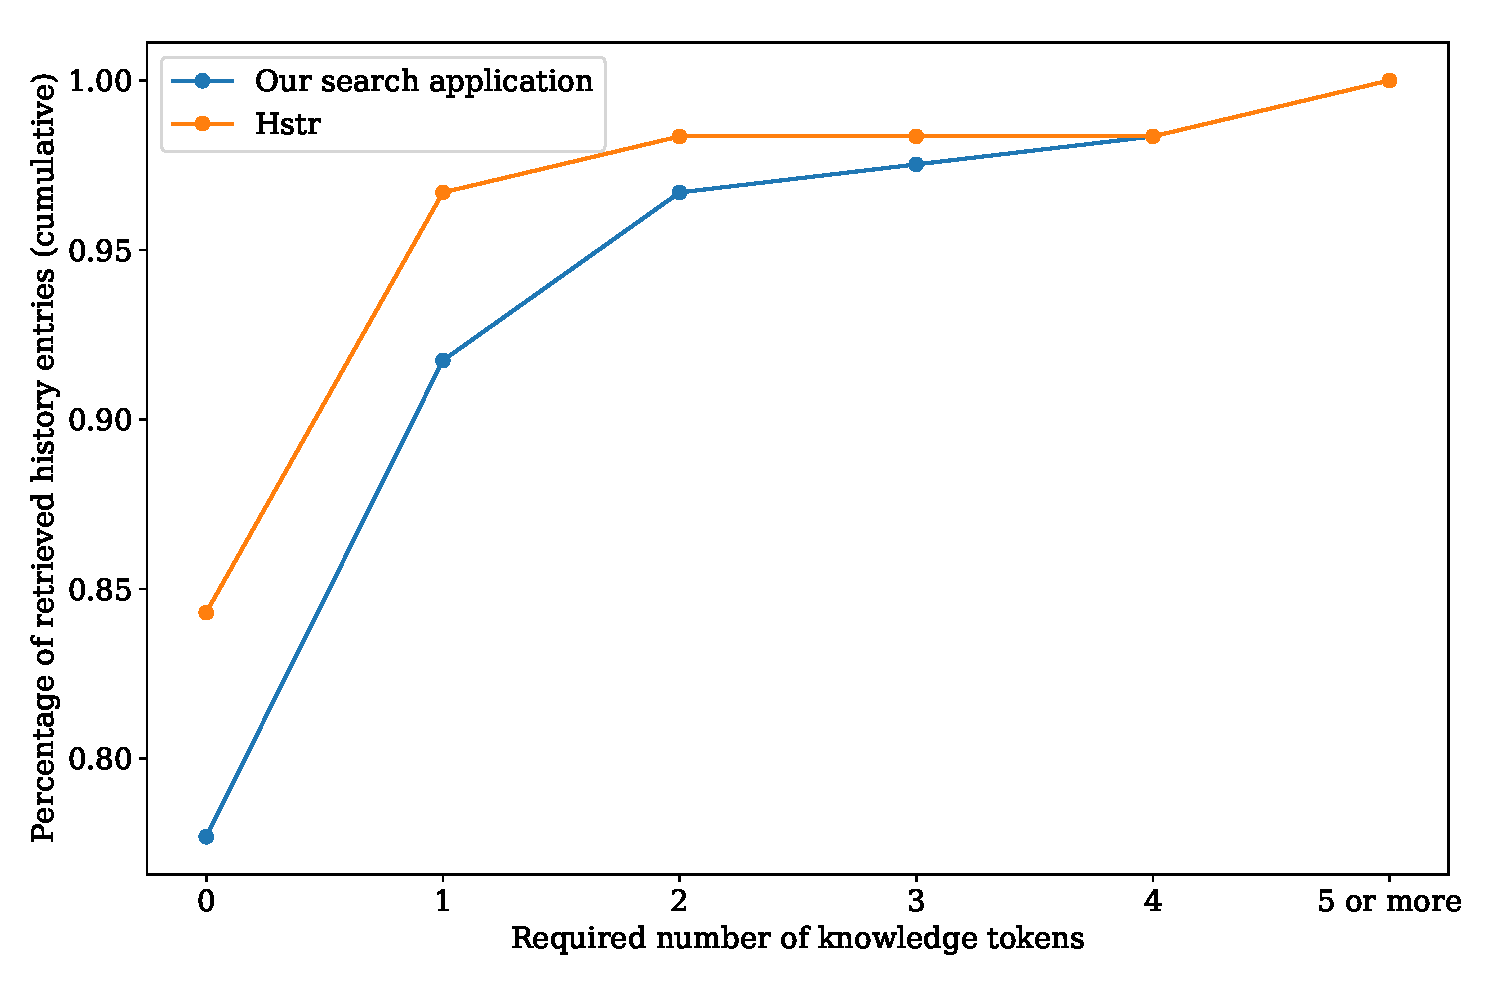
\includegraphics[width=0.5\linewidth]{figures/testing/testing-metrics-cmds-hstr.pdf}}\hfill
\tmpframe{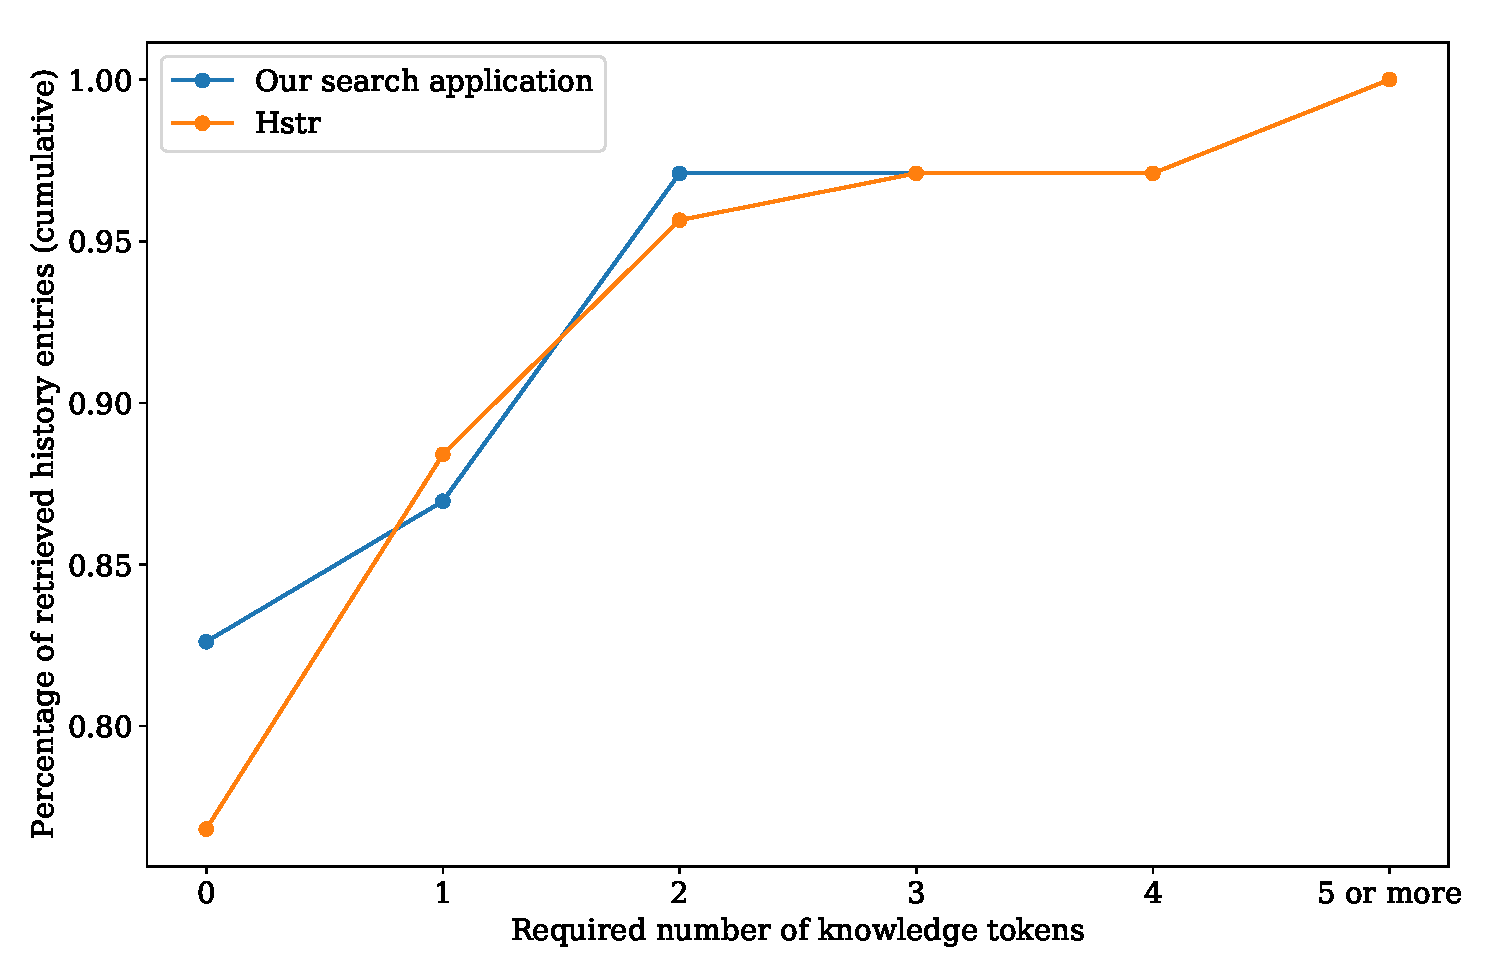
\includegraphics[width=0.5\linewidth]{figures/testing/testing-metrics-cmds-resh.pdf}}
\caption{Achievable searches as a function of knowledge (more is better)}
\small{Originally usage of Hstr (left) and usage of our search application (right)}
%\caption{Percentage of achievable searches (Originally performed using Hstr)}
\label{eval-metrics-plot-cmds}
\end{figure}

\begin{figure}[h!]
\centering
\tmpframe{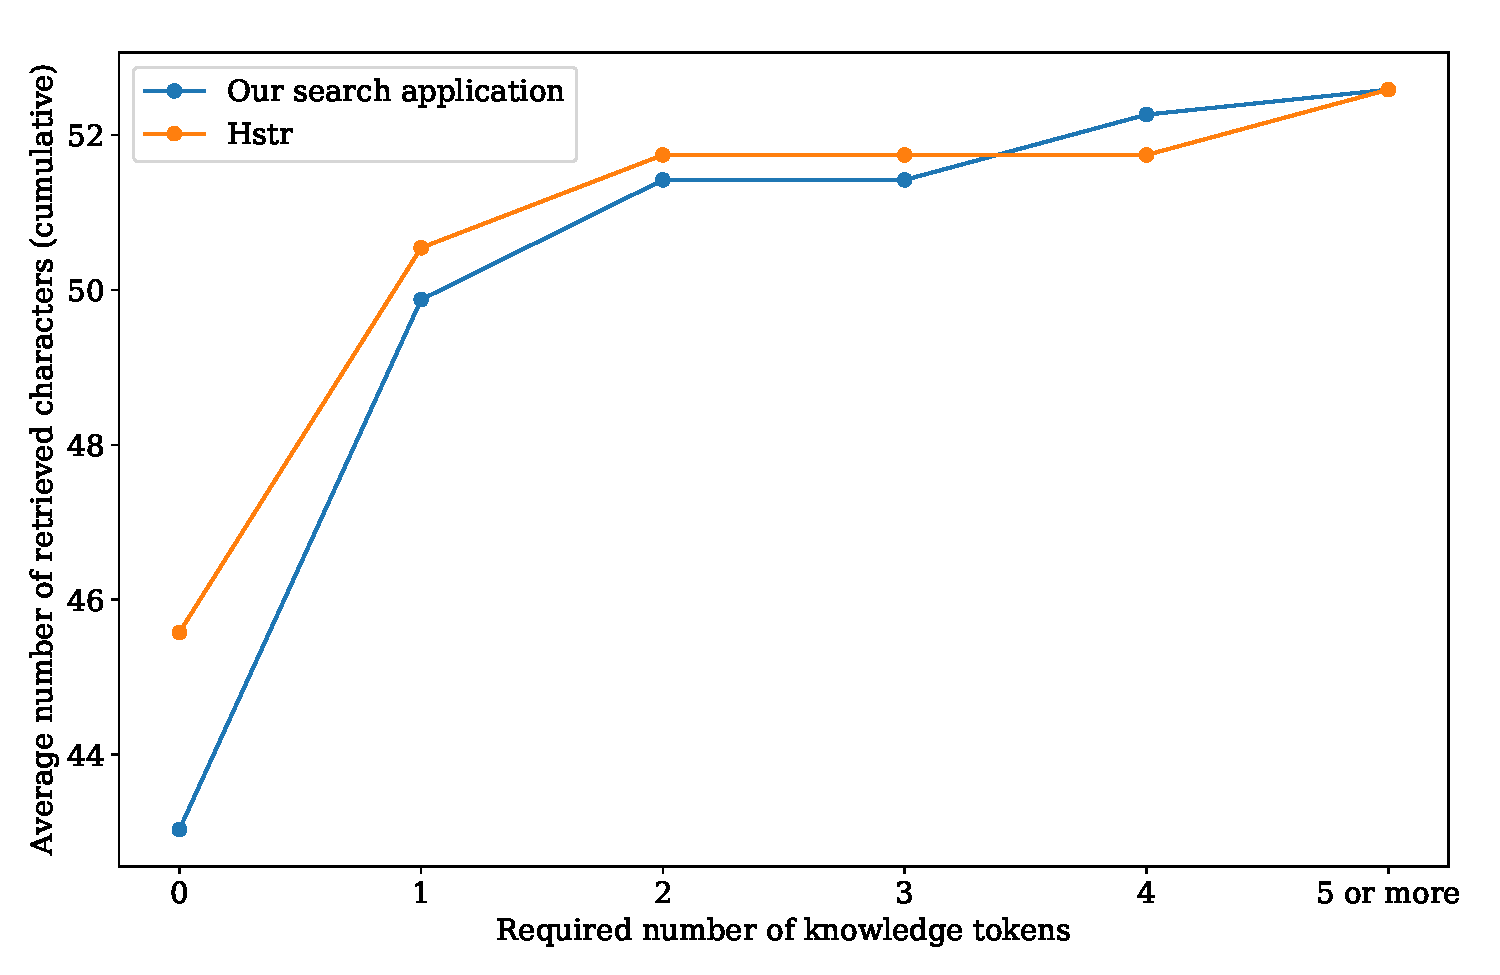
\includegraphics[width=0.5\linewidth]{figures/testing/testing-metrics-chars-hstr.pdf}}\hfill
\tmpframe{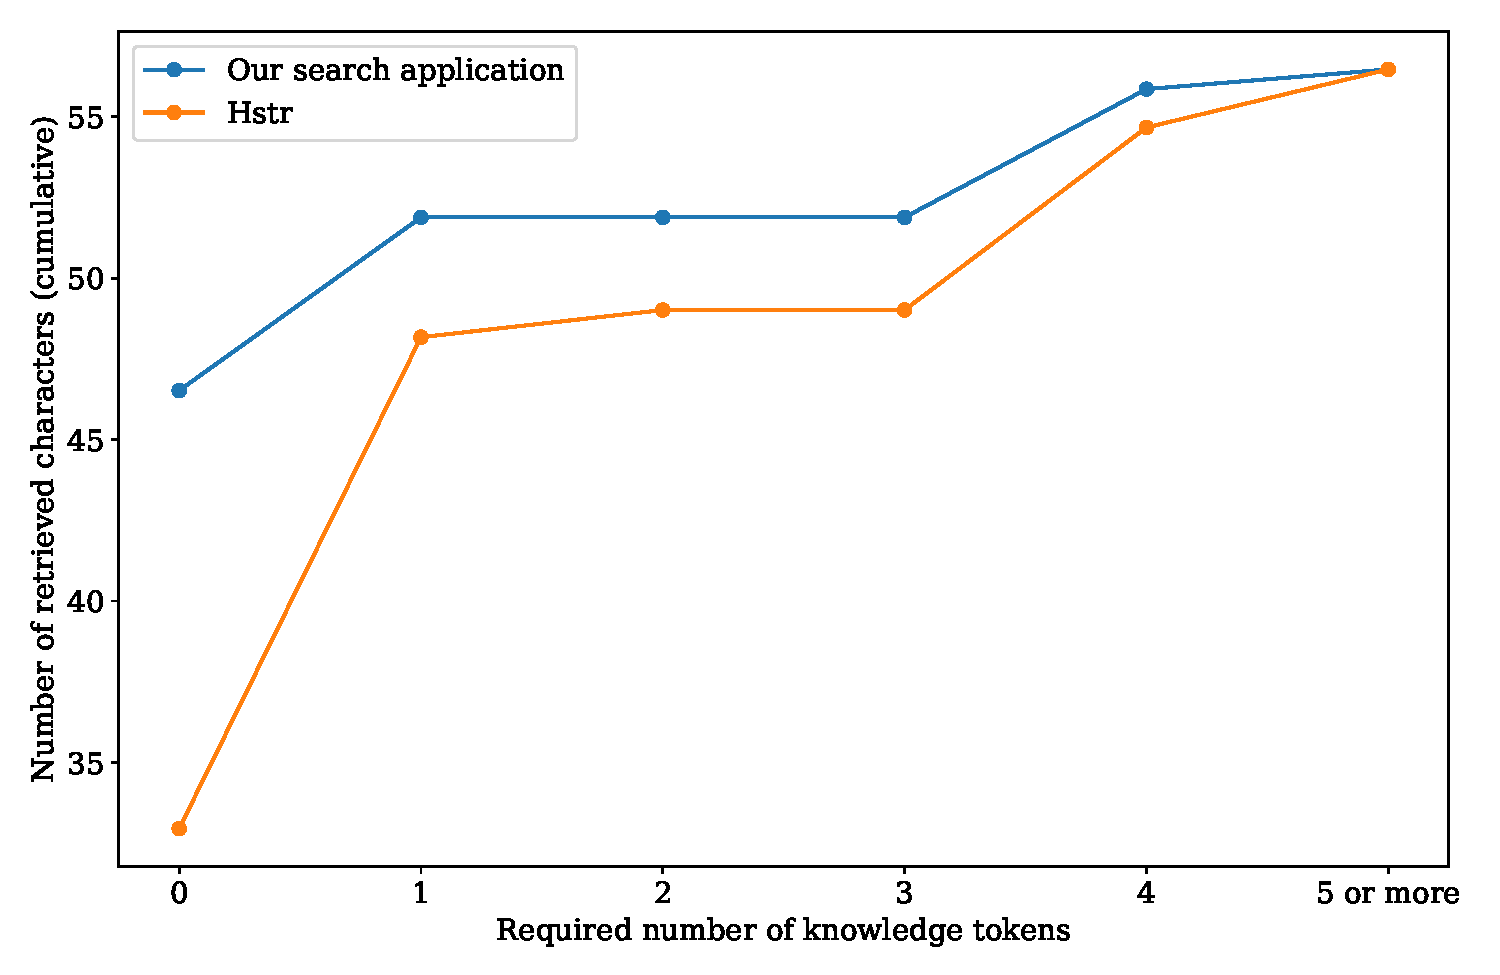
\includegraphics[width=0.5\linewidth]{figures/testing/testing-metrics-chars-resh.pdf}}
\caption{Avg. saved characters as a function of knowledge (more is better)}
\small{Originally usage of Hstr (left) and usage of our search application (right)}
\label{eval-metrics-plot-chars}
\end{figure}


\paragraph{Average saved characters as a function of knowledge}

Again, we are looking at how many searches are achievable for a limited number of knowledge tokens. However, we are also taking the length of the retrieved history entries into account. Essentially, searches that retrieve longer entries are worth more than shorter ones.

% In the previous section, each search was worth the same; Here, the searches retrieving longer history entries are worth more than ones retrieving short entries.

In figure \ref{eval-metrics-plot-chars}, we can observe many of the same characteristics as we saw in previous figure \ref{eval-metrics-plot-cmds}. Both history tools perform similarly in situations when the user originally used Hstr (left part of figure \ref{eval-metrics-plot-chars}). Our search application performs significantly better in situations when it was originally used (right part of figure \ref{eval-metrics-plot-chars}). 

When we compare figure \ref{eval-metrics-plot-cmds} with \ref{eval-metrics-plot-chars}, we can see that the difference between our solution and Hstr is more substantial when we take retrieved characters into account. 

Our application not only achieves more searches with limited knowledge; It also returns longer history results on average.

The fact that contextual history yields longer history entries is not surprising; It matches findings from previous research\cite{greenberg1993computer} where directory sensitive history returned longer history entries then simple recency-based history. More specific history entries generally tend to be longer, and generic and common command line entries tend to be shorter. 


\subsection{Position of results on the screen}

We had shown the difference between situations when the user originally used Hstr and when he used our search application. We have also explained why our application starts behaving similarly to Hstr as we increase the number of words we use as a query.

The main difference in performance between Hstr and our search application happens when we only search using little or no knowledge. Because of that, we further explore how the two history tools perform when searching with limited knowledge.

In this section, we are testing how many searches we can complete and how close to the top of the screen retrieved results show up. 

\paragraph{Achievable searches with zero knowledge}

Here, we want to find out how many searches are achievable if we only accept results from a given number of top positions. We are not using any query because we need to find out how well the search tools work when the user remembers nothing.

Figure \ref{eval-metrics-plot-dist-0-cmds} shows the percentage of searches that we could achieve if we only accepted results from a limited number of top positions on the screen. In other words, how many searches can we complete if we are only accepting results from, for example, the first ten returned results?

We can see that the performance of both history tools is similar in situations when the user originally used Hstr (left part of figure \ref{eval-metrics-plot-dist-0-cmds}). We will see this in all figures in this section. To not repeat ourselves, we are not going to mention it anymore.

As shown by the right part of figure \ref{eval-metrics-plot-dist-0-cmds}, Hstr and our solution perform similarly if we only accept results from the first nine positions (or less). If we accept results further down the screen, our solution is able to complete significantly more searches than Hstr.

Figure \ref{eval-metrics-plot-dist-0-chars} is very similar to figure \ref{eval-metrics-plot-dist-0-cmds}. It shows the average saved characters instead of the percentage of searches. All of the previous observations still hold. The performance differences between our solution and Hstr are more pronounced. 


\begin{figure}
\centering
\tmpframe{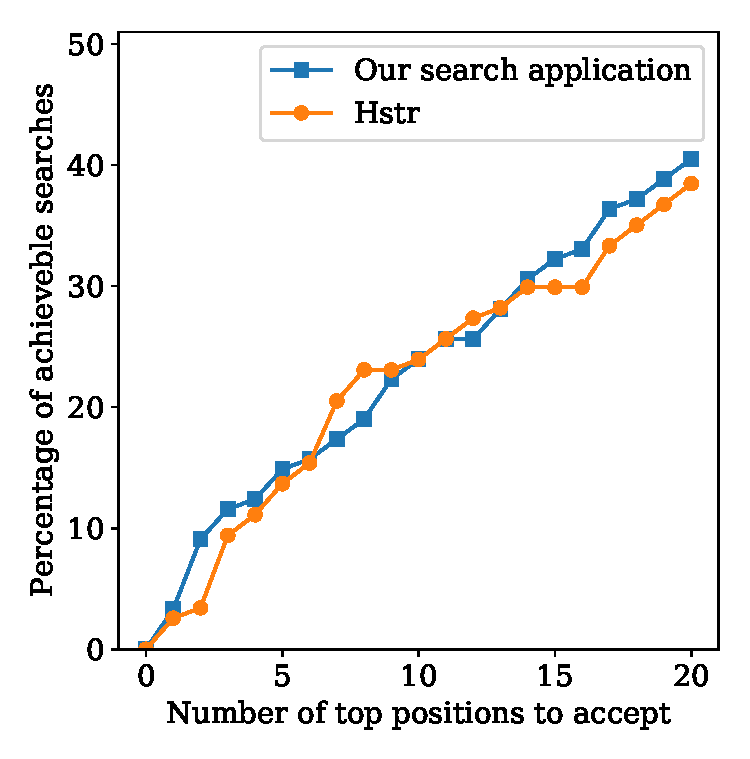
\includegraphics[width=0.5\linewidth]{figures/testing/testing-metrics-dist-0-cmds-hstr.pdf}}\hfill
\tmpframe{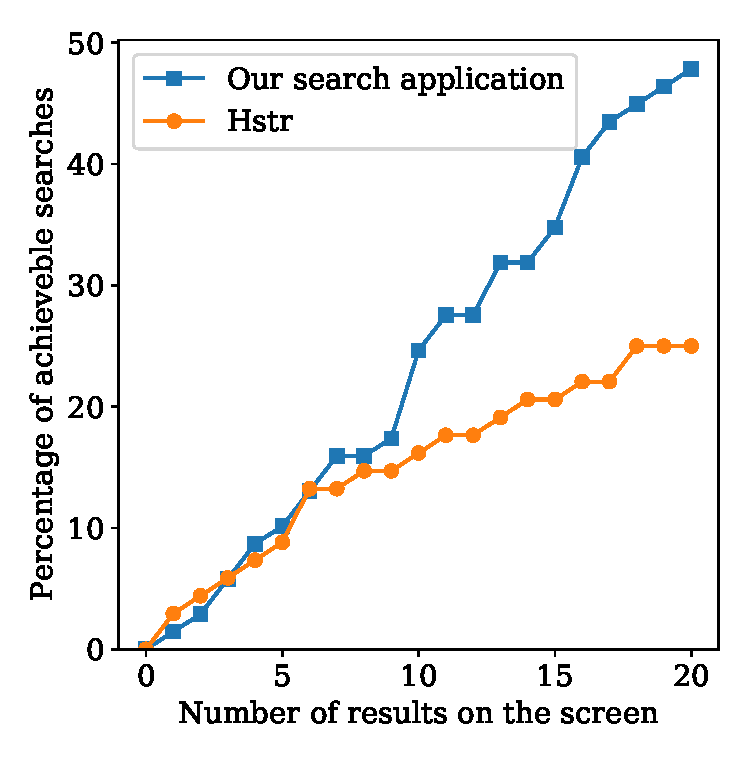
\includegraphics[width=0.5\linewidth]{figures/testing/testing-metrics-dist-0-cmds-resh.pdf}}
\caption{Achievable searches with zero knowledge (more is better)}
\small{Originally usage of Hstr (left) and usage of our search application (right)}
\label{eval-metrics-plot-dist-0-cmds}
\end{figure}

\begin{figure}
\centering
\tmpframe{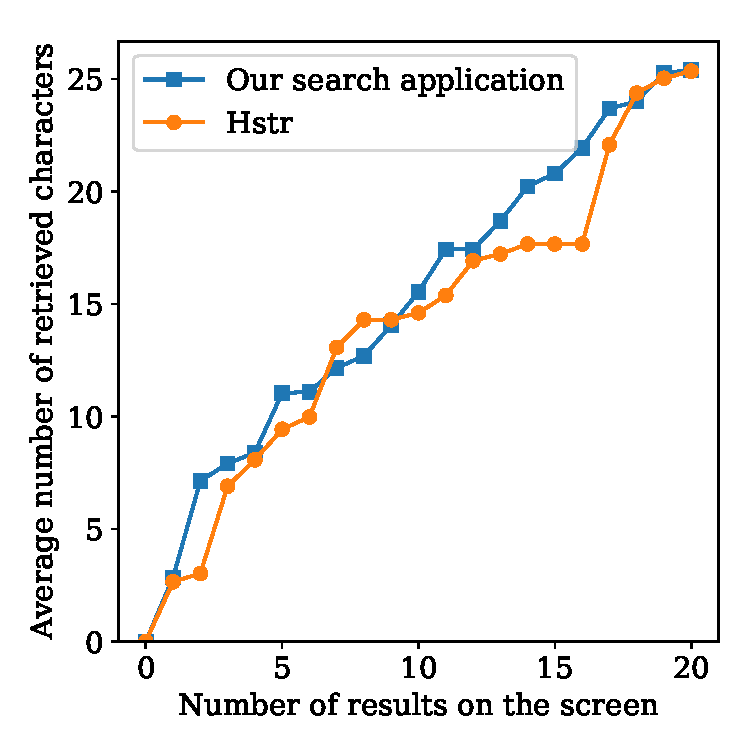
\includegraphics[width=0.5\linewidth]{figures/testing/testing-metrics-dist-0-chars-hstr.pdf}}\hfill
\tmpframe{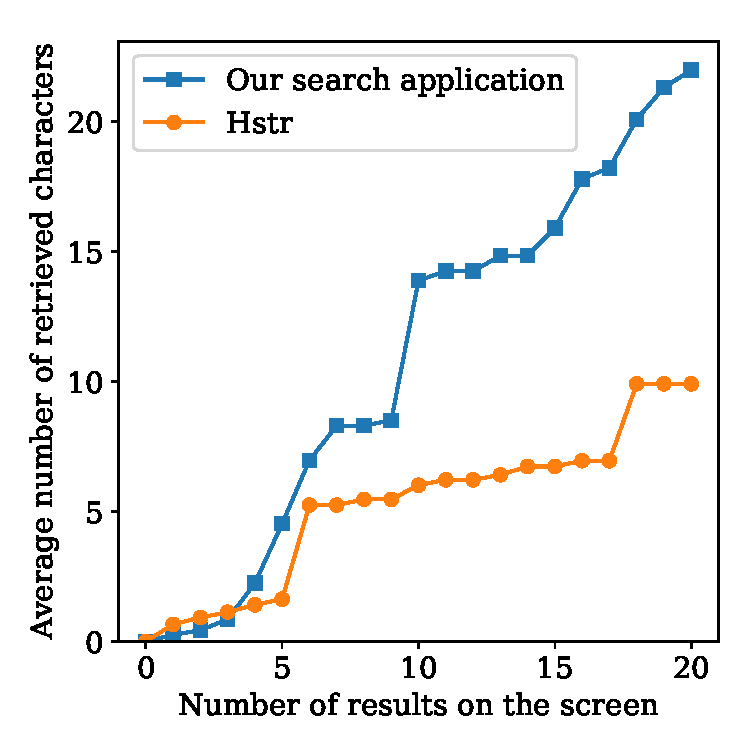
\includegraphics[width=0.5\linewidth]{figures/testing/testing-metrics-dist-0-chars-resh.pdf}}
\caption{Average saved characters with zero knowledge (more is better)}
\small{Originally usage of Hstr (left) and usage of our search application (right)}
\label{eval-metrics-plot-dist-0-chars}
\end{figure}


\newpage
\paragraph{Achievable searches with a single word query}

Once again, we are interested in finding out how many searches are achievable if we only look at a given number of top results. This time, however, we provide a single knowledge token as a query to the search tools.

As shown by the right part of figure \ref{eval-metrics-plot-dist-1-cmds}, our search application can complete more searches than Hstr. Now that we provide a query to the searching tools the difference is less striking (compare figure \ref{eval-metrics-plot-dist-0-cmds} and \ref{eval-metrics-plot-dist-1-cmds}). We can see how even a single query word has a serious influence over the scoring function and, by extension, displayed results. 

Right part of figure \ref{eval-metrics-plot-dist-1-chars} shows a significant difference between Hstr and our solution. Hstr retrieves much shorter history entries than our search application. Our application saves considerably more typing to the user when a single word query is used. 

\subsection{Evaluating metrics}

We conclude that our history search application and Hstr perform similarly in all tasks that the user originally performed using Hstr. Contrarily, Hstr does not perform well in all situations when our application can be used. It appears that our solution covers extra workflows that are more difficult to achieve with Hstr. Examples of such workflows are described in the previous section \ref{test-real-life-scenarios}. 
%It seems that users learn what their tools can or cannot do and use them accordingly.

Our search application enables users to retrieve history entries with less typing and remembering. Specifically, with no query, Hstr can only complete about half of the number of searches our solution can. 

Furthermore, our search application, on average, retrieves longer history entries from history. Longer history entries take longer to type and remember. This means that the average effort saved to the user should be higher when using our solution. 

We should point out that we have used the same full shell history for both Hstr and our search application. Hstr normally uses standard shell history, which might be missing some history entries. In reality, we expect the performance of Hstr to degrade because of the missing history entries.

\begin{figure}
\centering
\tmpframe{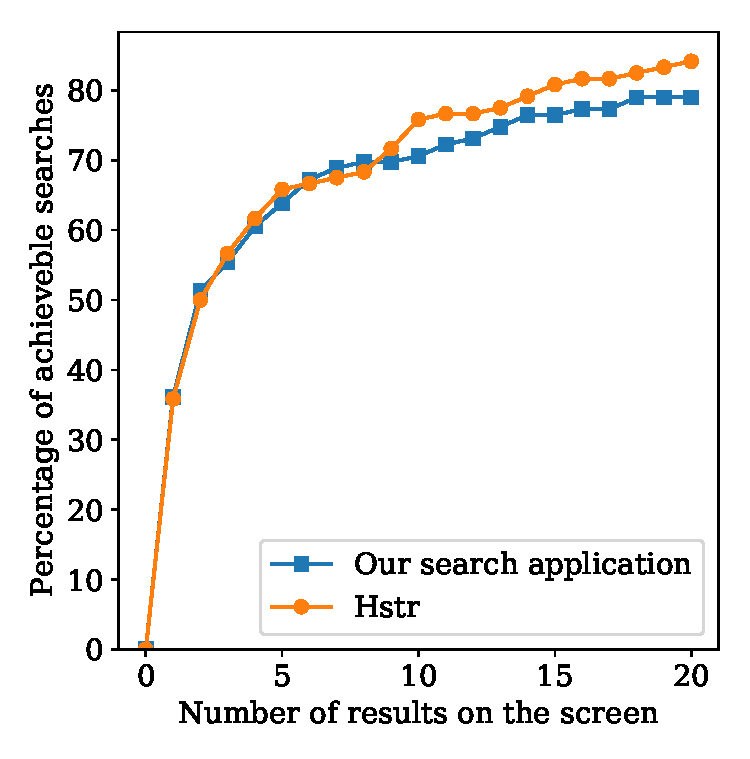
\includegraphics[width=0.5\linewidth]{figures/testing/testing-metrics-dist-1-cmds-hstr.pdf}}\hfill
\tmpframe{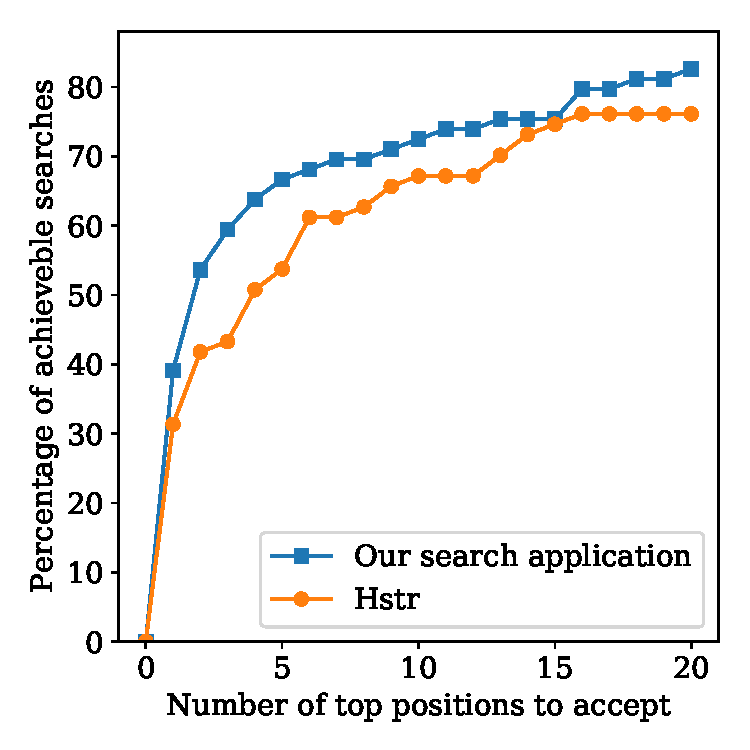
\includegraphics[width=0.5\linewidth]{figures/testing/testing-metrics-dist-1-cmds-resh.pdf}}
\caption{Achievable searches with a single knowledge token (more is better)}
\small{Originally usage of Hstr (left) and usage of our search application (right)}
\label{eval-metrics-plot-dist-1-cmds}
\end{figure}

\begin{figure}
\centering
\tmpframe{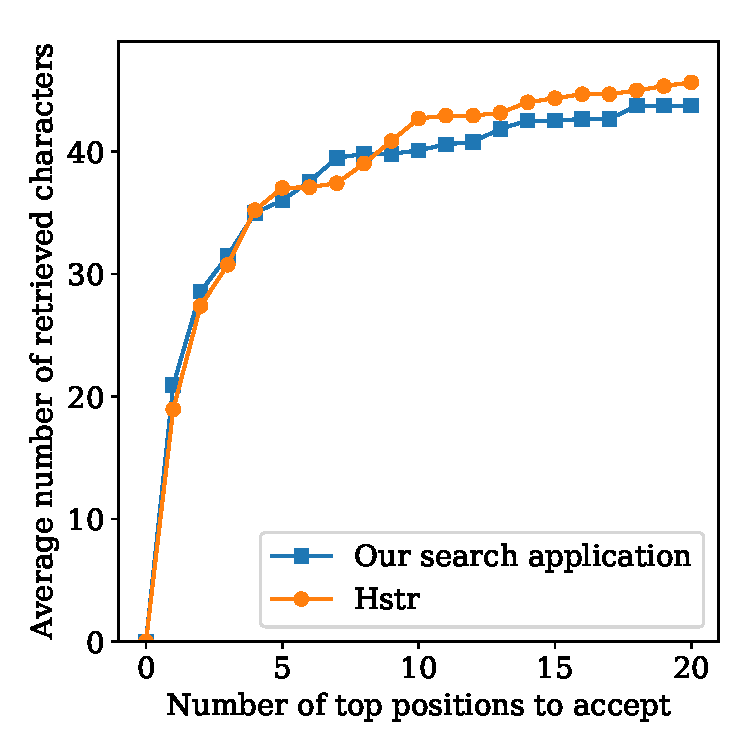
\includegraphics[width=0.5\linewidth]{figures/testing/testing-metrics-dist-1-chars-hstr.pdf}}\hfill
\tmpframe{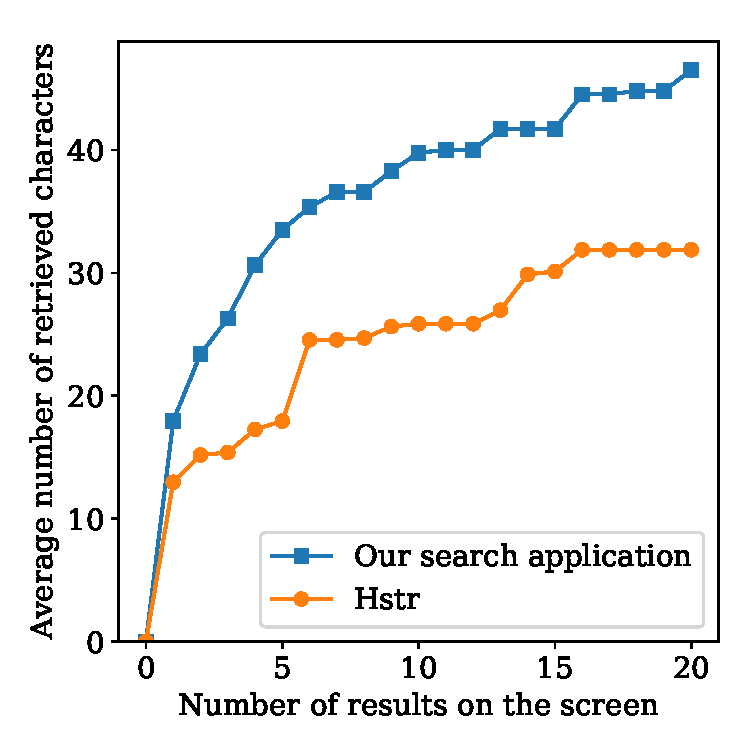
\includegraphics[width=0.5\linewidth]{figures/testing/testing-metrics-dist-1-chars-resh.pdf}}
\caption{Avg. saved chars. with a single knowledge token (more is better)}
\small{Originally usage of Hstr (left) and usage of our search application (right)}
\label{eval-metrics-plot-dist-1-chars}
\end{figure}

\section{User feedback}

In this section, we describe how we released the project to the public, what improvements we made based on interviewing our users, and what feedback we get from users,

We released the first prototype of the search application about four months ago. Since then we are engaging with our users and incrementally updating and improving the project. 

\subsection{User adoption}

Since the release of the first prototype of the search application four months ago, the project was downloaded and installed over 600 times. 

The project also received over 250 stars on GitHub which is a bookmarking and endorsement feature on the GitHub website.\cite{github-stars}\cite{resh-github-homepage}


\subsection{Feedback from the users}

Here, we describe what improvements we made to the project and what feedback we got from our users. We only mention a few examples of changes and feedback.

\paragraph{Non-contextual mode}

Some of the users were asking for a way to turn off the contextual search because it can occasionally get in their way. For example, logging into remote servers with \verb|ssh| can be done regardless of the current directory. When searching for past \verb|ssh| commands, the contextual search might do more harm than good.

Based on this, we have added the ability to switch between contextual and non-contextual mode with \verb|CTRL-R|. This way, the user can always choose the appropriate tool for the specific situation. A screenshot of the non-contextual mode is shown in figure \ref{xterm-resh-raw-80}.

\begin{figure}
\permanentframe{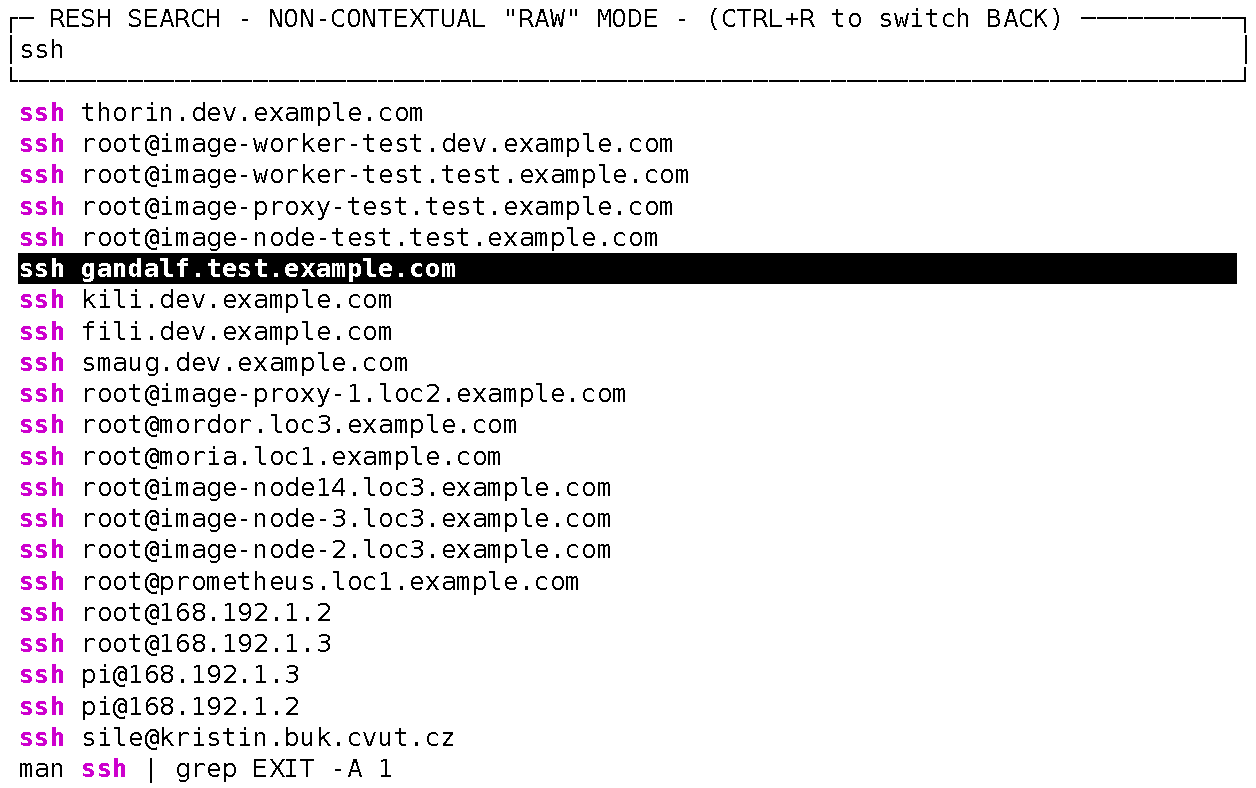
\includegraphics[width=0.995\linewidth]{figures/testing/xterm-resh-raw-80.pdf}}
\caption{Screenshot of the non-contextual mode of the search application}
\label{xterm-resh-raw-80}
\end{figure}

\paragraph{More ergonomic arrow key bindings}

One of our users was complaining that he is used to repeatedly pressing \verb|CTRL-R| to navigate to between the search results. He was previously using the standard reverse search.

By interviewing the user, we have discovered that he would like more ergonomic key bindings for arrow keys. He does not like reaching to the arrow keys from the home row. We have added alternative Emacs-inspired bindings for arrow keys; Pressing \verb|CTRL-N| selects the next result on the page and \verb|CTRL-P| selects the previous one. 


\paragraph{Special handling for exit status}

We got some feedback regarding using exit status as part of contextual search. When users kill the running command using \verb|CTRL-C|, it exits with the status of 130.
We anticipated that this would happen, but it is more common than we expected.
We could add special handling for exit statuses that have special meaning. This feature, however, is not included in the current release.

%\redtext{SKIP ?}
%\begin{itemize}
% \item Better help / onboarding
% \item Directory jumping - history vs. specialised tools
%\end{itemize}


\subsection{User testimonies}

Now, we sum up what people say about the project. 

In our user base, we have people who have switched from Hstr to our history system. Multiple people have said that our search application has fully replaced Hstr in their workflows. It seems that we provide a reasonable alternative to Hstr.

We shared the project online on multiple occasions, and the feedback we received from people was overwhelmingly positive.\cite{resh-feedback}\cite{resh-feedback2}

\section{Additional workflows}

In this section, we describe additional workflows that are possible to complete using our search application. 

\subsection{Quickly retrieve history from other sessions}

Since standard history is handled individually in each session, users cannot access history from other simultaneously running sessions. 

Our search application uses history from all running sessions immediately. This means that users can quickly access history from other open terminals. 

Specifically, pressing \verb|CTRL-R| twice launches the search application and switches to non-contextual mode; This way, the user can see all recent history entries from all sessions.

\subsection{Find similar history entries}

When the search application is launched, the contents of the command line are used as the initial query. For example, the user can use \verb|ARROW_UP| to retrieve the previous history entry and then press \verb|CTRL-R|. 

Using a full command line entry as a query fills the page with similar history entries. This is possible because of the properties of our scoring function; It returns reasonable results even when there are words in the query that do not match anything. 

\subsection{Write new command line entries based on history}

Sometimes we want to write a new command line entry, but we do not quite remember all of its parts. Seeing similar history entries as we type, could make constructing the new entry much easier.

As we already mentioned, when launching the search application, the contents of the command line are used as a query. Conversely, the user can press \verb|CTRL-G| to abort the search, and the contents of the query are pasted back onto the command line.
Combining these two actions makes it possible to transfer back and forth between the command line and the search application. 

%All this can be used to write new command line entries while

We can launch the search application and start writing the command line entry into the query field. The search application continuously shows us similar history entries we can use as an inspiration. When we are done with typing the command line entry, we use \verb|CTRL-G| to get back to the command line. Then, we can execute the command line entry.


\section{Evaluation conclusion}

Here, we sum up our findings from testing and evaluating our history searching solution. We point out why our search application is a useful replacement for both standard reverse search and Hstr. 

Our search application matches the usability improvements that Hstr offers compared to the standard reverse search. We have shown this using chosen real-life scenarios.

There are tasks that the observed user completed using Hstr. Our search application matches the searching performance of Hstr in all of those situations. This means that using our solution instead of Hstr does not lead to degraded performance.

There are new workflows that are easier to perform using our search application. Hstr does not perform well in those situations. Real-life examples of such situations are described in section \ref{test-real-life-scenarios}.

Our solution can complete more searches with less knowledge and typing compared to Hstr. If the user switched back to Hstr, he would have to use queries in about half of all searches that are possible with zero knowledge in our search application. Our search application also retrieves longer history entries, which saves more typing and remembering to the user.

Depending on a specific situation, the average performance of our search application is either comparable to or better than Hstr. In many situations, however, our solution performs significantly better than Hstr. Because of that, we conclude that the contextual search is a great default way to search history. Furthermore, users have the option to switch between contextual and non-contextual mode. This is useful for retrieving history entries that are clearly non-contextual.
We released the first prototype of the search application about four months ago. Since then, the application has grown in popularity, and it was installed over 600 times. We have received overwhelmingly positive feedback. There are people who switched from Hstr to our search application and said that our solution has entirely replaced all their Hstr workflows.



